\documentclass[journal]{IEEEtran}

% Packages
\usepackage{cite}
\usepackage{graphicx}
\usepackage{subfigure}
\usepackage{float}
\usepackage{url}
\usepackage{color}


\begin{document}

% paper title
% can use linebreaks \\ within to get better formatting as desired
\title{Probabilistic~Robotics~Lab~3 \\ Particle~Filter}
%

\author{Rodrigo~Caye~Daudt}





% make the title area
\maketitle



%%%%%%%%%%%%%%%%%%%%%%%%%%%%%%%%%%%%%%%%%%%%%%%%%%%%%%%%%%%%%%%%%%%%%%%%%%%%%%%
\section{Introduction}

\IEEEPARstart{T}{his} report describes the work done for lab 2 on the Probabilistic Robotics module, for which a particle filter was developed in Python to work with ROS simulations. Section \ref{pf} describes the workings of a particle filter and gives some information about our implementation. Section \ref{results} shows and analyses the results obtained by using the developed filter. Section \ref{conclusion} closes this work with the main observations and conclusions.

%%%%%%%%%%%%%%%%%%%%%%%%%%%%%%%%%%%%%%%%%%%%%%%%%%%%%%%%%%%%%%%%%%%%%%%%%%%%%%%
\section{Particle Filter}\label{pf}

The particle filter, also known as Monte Carlo Localization, is a genetic type algorithm used to keep track of the location and position of robots. The main idea behind this algorithm is to substitute the operations with probability density functions (PDFs) used in the Bayes filter by a set of weighted samples of that same function.

By using a sampled version of the PDF we can avoid complex calculations of prediction and correction over all configuration space. We can instead simply apply the prediction and correction steps directly to each particle, which is a much simpler operation than dealing with PDFs. On the other hand, this sampling makes it necessary to carry out these operations for each sample, therefore the number of simulated particles will be defined by how much computing power we have available. The usage of more particles leads to a more stable system.

The particle filter is divided in three main steps: prediction, weight update, and resampling. These steps may or may not be carried out in order during the robot's operation. The prediction step is carried out once odometry data is available, since it allows us to predict the movement of the robot, or of the particles in this case. The weight update step is carried out when sensor data is obtained to evaluate the validity of our predicted values. Finally, the resampling step is done when the weights have drifted far from the initial given weights.

The prediction step is simply using the motion data obtained from the odometry sensors to update the position of the particles. It is important to keep in mind in this step that the odometry data has a different meaning for each particle, given that this data is dependent on the position and orientation of the robot. The state of each particle is updated as if the robot was in that state, and then a small amount of noise is added to the new state to add some variability to our system. Without the addition of independent noise, particles in the same state (which is very likely to happen after the resampling step) would stay together from that moment onwards and multiple calculations would be meaningless. This added noise helps us deal with the imprecision of the odometry sensors of the robot.

The weight correction step is carried out once we have data from the robot's sensors relative to the environment. This model is used along with an environment model and the weight of each particle is updated according to how well the observations confirm the state of a given particle. After this step, particles which seem more likely to be close to the true state of the robot will have a higher weight than the others. In our case, this was accomplished by comparing the measured lines from the laser scanner to the lines of a map of the environment the robot was placed in. After converting the lines to the distance/angle form, the lines were compared to the lines in the map and the best fit was considered to update the weight of that particle. The weight of each particle was updated by a factor $w$ defined by Eq. \ref{eq:w}, where $x$ is the measured value, $\mu$ is the expected value, and $\sigma$ is the standard deviation of that measurement. The value of $\sigma$ can be used as a tuning parameter, since a lower value of $\sigma$ means we have a higher trust level in our measurement. This equation was applied separately for range and angle of the lines, and both results together defined which line was the best match.

\begin{equation}\label{eq:w}
w = \frac{1}{\sigma \sqrt{2\pi}}exp\Bigg[-\frac{(x-\mu)^2}{2\sigma ^2}\Bigg]
\end{equation}

An extra step was added to update the weights of the particles. Since the lines in the form of distance/angle have no boundary, the sizes of the lines can not be considered in this way. Being so, the length of the measured lines were compared to the length of its best match in the map data, and if the length of the measured line was larger than the length of the map line the weight of the particle was set to zero, since it meant that the particle was lost. A tolerance of $10\%$ was used for the comparison of the lines since the laser measurements may not be very precise, especially when coupled with line extracting algorithms.

Finally, the resampling of the particles was done only when the weight of the particles drifted too far from the initial values. This drifting was measured by the $\hat{N}_{eff}$, which is defined in Eq. \ref{eq:neff}. The resampling was done using the low variance sampler algorithm. The resampling was computed when $\hat{N}_{eff}$ dropped below a threshold of $number\_of\_particles/2$.

\begin{equation}\label{eq:neff}
\hat{N}_{eff} = \frac{1}{\sum_{L=1}^{M} \Big(w_k^{(L)}\Big)^2}
\end{equation}






%%%%%%%%%%%%%%%%%%%%%%%%%%%%%%%%%%%%%%%%%%%%%%%%%%%%%%%%%%%%%%%%%%%%%%%%%%%%%%%
\section{Tests and Results}\label{results}

The developed particle filter was tested using recorded data of a real robot test and using a simple map representation of the environment where it was placed. This allowed us to evaluate the behaviour of our algorithm in a real word situation, even if the data stream was not live. The simulations were run using 500 particles for our filter.

We can see in Fig. \ref{initial} the initial configuration of the particles and the robot represented in yellow. The particles were initialized around the position of the robot with an offset of $[-1,1]$ in the X and Y axes. The orientation of the initial particles was initialised completely at random. This initialization implies that we had some prior knowledge of the position of the robot, but not of its orientation. We can also observe that the weights at this point are all equal, since they have not been updated at this point.



\begin{figure}[H]
	\centering
	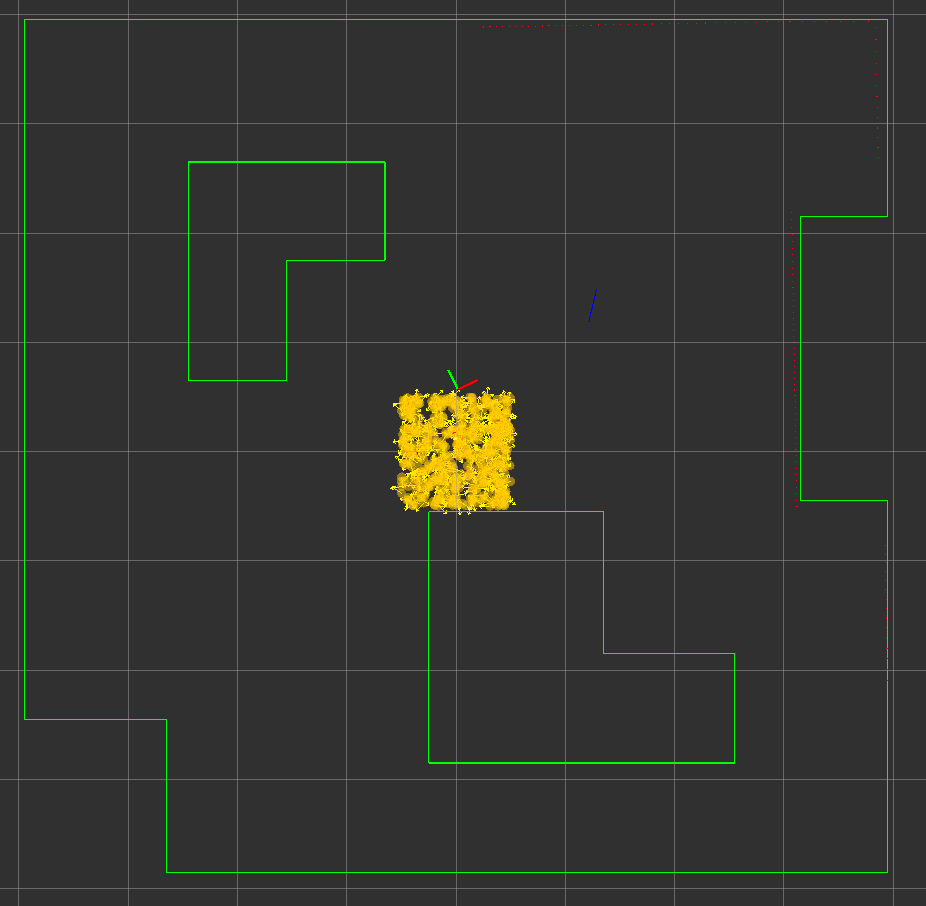
\includegraphics[width=0.8\linewidth]{figures/initial.png}
	\caption{Initial configuration of particles in test environment}
	\label{initial}
\end{figure}

The prediction, weight update and correction steps were executed in fast succession so it's hard to separate their results, but we could see that all processes working together led to the particles grouping together and following the robot. This proves that the particle filter is able to reject incorrect particles by using the information from the extrinsic sensors. When the program was running, the particles became aligned almost instantly. It was observed that some ambiguity occurred with the provided map, since it was common for the particles to split into two groups at the beginning of the simulation. This is not a flaw of the algorithm, but merely a consequence of the random initialization of the particles coupled with the ambiguity of the map measurements.

Figure \ref{final} shows the result of the simulation after the robot had circled the whole room (using all the available recorded data). We can see the position and orientation of the mean particle over several steps along the simulation displayed. While it's hard to exemplify with pictures, it was easy to observe during the simulation how well the particle filter was performing. The only flaw was that there was a small delay between the robot movement and the update of the particle filter, which could be a problem for high precision applications.


\begin{figure}
	\centering
	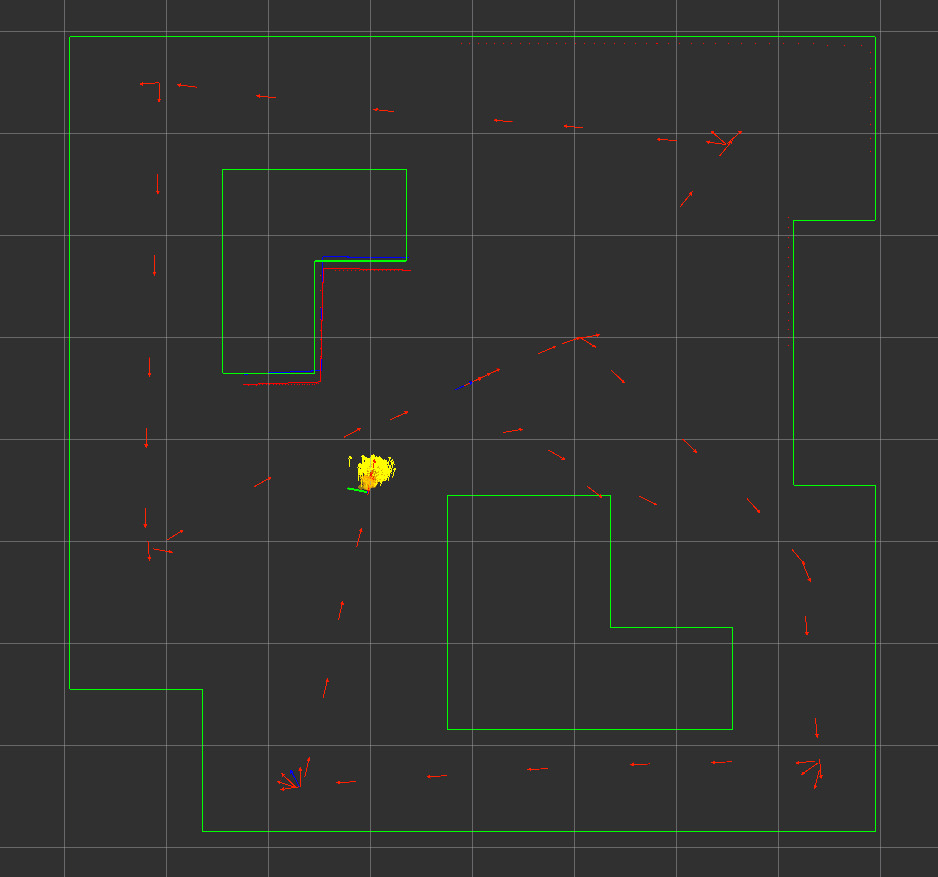
\includegraphics[width=0.8\linewidth]{figures/final.png}
	\caption{Trajectory taken by the particles using the measurement information on a successful run}
	\label{final}
\end{figure}

Finally, it was observed that the addition of the extra step described at the end of Section \ref{pf} caused some instability in the filter on this particular simulation. More simulations with different environments could help to define whether or not this step was actually helpful for our filter. This instability was counteracted by multiplying the value of $\sigma$ in Eq. \ref{eq:w} by a tuning factor. Doing so decreased our trust in our measurement and kept our particles for longer before they were removed through resampling.




%%%%%%%%%%%%%%%%%%%%%%%%%%%%%%%%%%%%%%%%%%%%%%%%%%%%%%%%%%%%%%%%%%%%%%%%%%%%%%%
\section{Conclusion}\label{conclusion}

We observed during the development of this work how a particle filter works. We were also able to bserve some of its advantages and disadvantages. The particle filter seems o be very stable once the particles have correctly identified the position of our robot, but some instability was observed during the initialization of the particles when all angles were randomly defined.

We also observed how fast the computations of the particle filter are. The way the filter was implemented did not lead to a very fast result, but it is possible that the code could be restructured to work in a faster way. One suggestion to accomplish this would be to compute the prediction step and the weight update step in matricial form using numpy instead of using for loops.

We concluded that particle filters are a good and simple to implement solution for solving the filtering problem as long as we have access to a reliable map from the beginning of the execution. We also observed that some conditions may lead to instability in the behaviour of this filter, so it must be tuned correctly.


%\bibliographystyle{IEEEtran}
%\bibliography{Template_Daudt}


\end{document}


